\documentclass[hyperref={pdfpagelabels=false},aspectratio=169]{beamer} \mode<presentation> { \usetheme{Boadilla} }
\setbeamertemplate{navigation symbols}{}

\title[Toy Studies]{Effective Area Studies with a Toy Generator}
\author{Cosmin Deaconu}
\institute{UChicago/KICP}

\begin{document} 

\begin{frame}[plain]
  \maketitle
\end{frame} 

\begin{frame}
\frametitle{Context} 
\begin{itemize} 
\item In the fall, I became worried that the $A_{eff} = V_{eff}/L_{int}$ approximation may not be right for a non-infinite disc geometry. 
\begin{itemize}
\item In the non-infinite disc case, cannot factor out the projected length from the trajectory. 
\item Also, two different generators for ANITA MC gave factor of two difference (much more complicated geometry there, though). One generator uses $V_{eff}/L_{int}$, the other computes $A_{eff}$ directly. 
\end{itemize}
\item So I wrote a toy MC to test the two generators. 
\end{itemize} 
\end{frame} 

\begin{frame} 
\frametitle{Toy MC} 
\begin{itemize}
\item \url{https://github.com/cozzyd/ToyDisc} 
\item From-scratch very basic Askaryan neutrino simulation in a cylinder of uniform ice, with two different generators and $A_{eff}$ procedures..  
\item Implements simple interaction / inelasticity / Askaryan emission model and electric field threshold at detector for trigger. 
\begin{itemize}
\item Conolly et al inelasticity, interaction model. 
\item Same Askaryan emission parameterization as used in \texttt{icemc} . 
\item Since uniform ice, no raytracing.  Use constant attenuation length. 
\end{itemize} 
\item \textbf{Can't compare effective areas with a real simulation} (due to simple trigger and uniform ice model). The point is to compare the two generators in a simple setup that can run fast (100 million events in about 10 minutes on my workstation). 
\end{itemize}
\end{frame}

\begin{frame}
\frametitle{Procedure A (the standard forced method)} 
\begin{itemize} 
\item Generate random direction and random position within cylinder. 
\item Compute ``absorption weight,", $w_a$: the chance of the neutrino not having interacted before entering the simulation volume. 
\begin{itemize} 
\item Use PREM model with ice layer on top. Generate histogram of column density vs. angle and depth for interpolation (and subtract off column density from entrance point in volume to interaction). 
\end{itemize} 
\item  Also keep track of interaction length for each neutrino (since flavor,charge-dependent). Leads to: 
\begin{equation}
  <A_{eff}>|_{\Omega}=  \left< \frac{V_{eff}}{L_{int}} \right>  = \frac{V_{mc}}{N} \sum_i \frac{w_{a,i}}{L_{int,i}} pass_i
\end{equation} 
\end{itemize} 
\end{frame}

\begin{frame}
\frametitle{Particle depth histogram} 
\centering
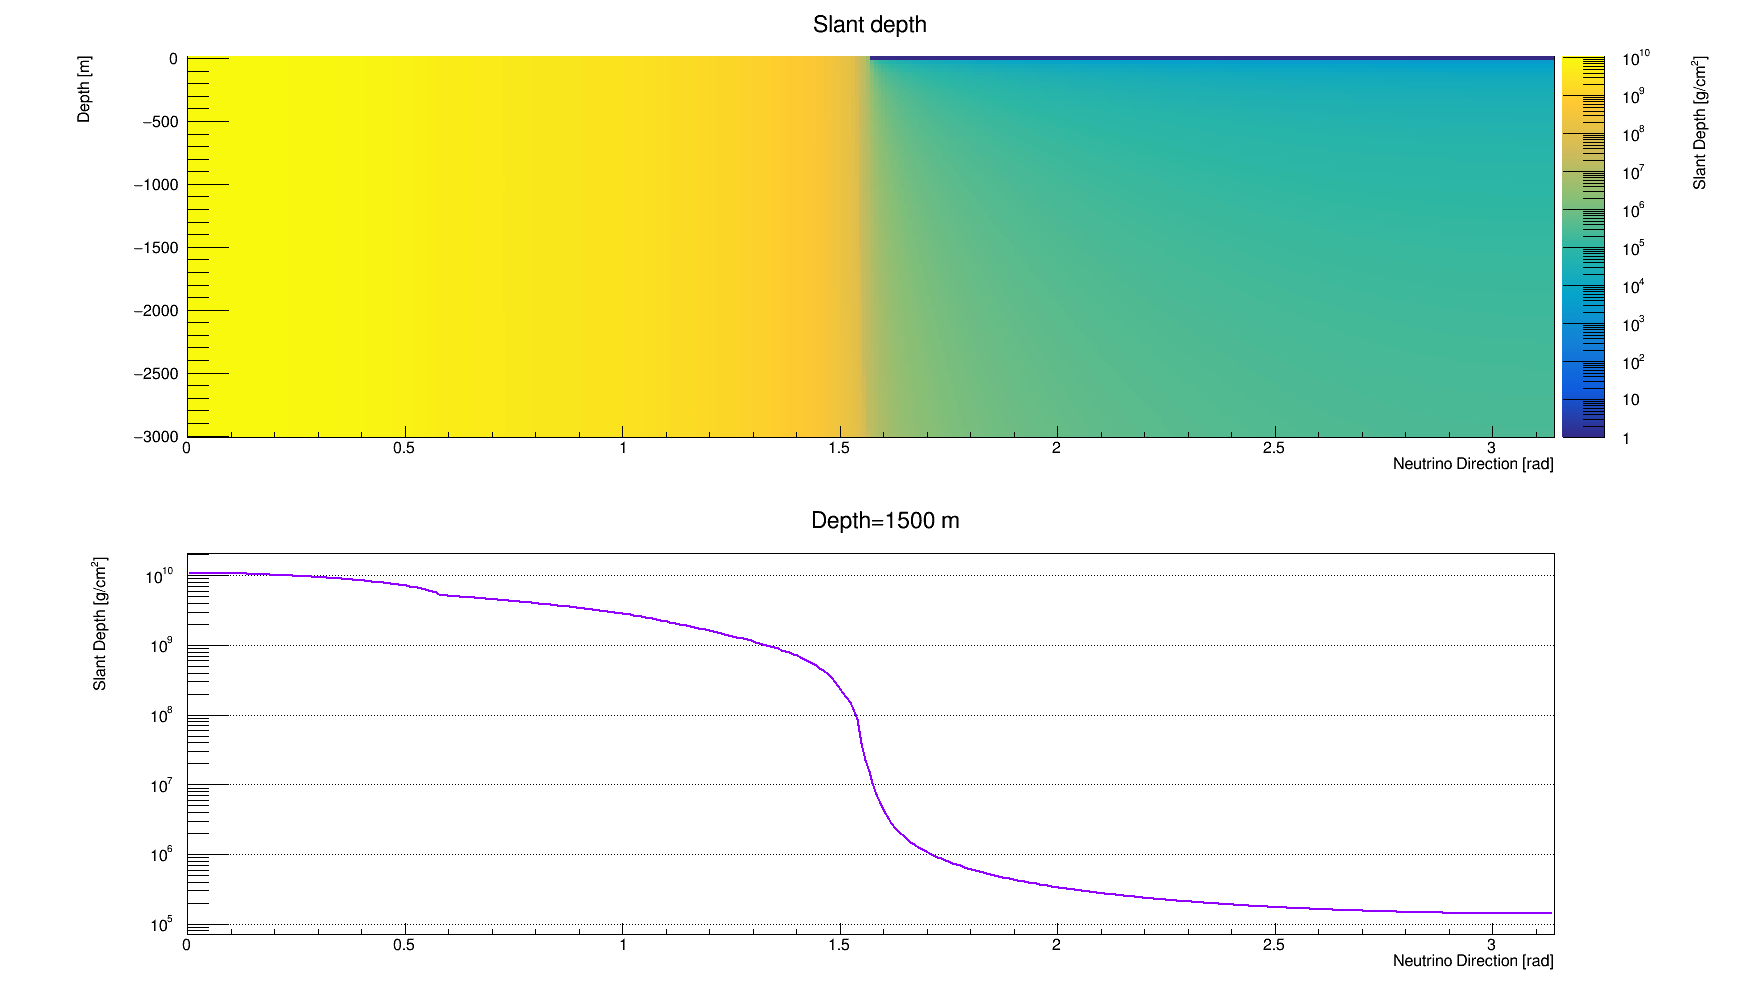
\includegraphics[width=5in]{slant_depth} 
\end{frame}

\begin{frame}
\frametitle{Procedure B (area method)} 
\begin{itemize}
\item Generate a random direction. 
\item Sampling area is a box  passing in center of volume normal to neutrino direction. Box is big to cover largest projected area ($L= \sqrt{4*R^2+h^2}$). Randomly pick offset within sampling box.
\item Check for intersection of trajectory with the simulation volume. If no intersection, then continue. 
\item If trajectory intersects volume, pick a point for interaction (exponential weighting, but linear would work fine too with the interaction lengths considered here) and calculate two weights: 
\begin{itemize}
  \item $w_a$, identical to before.
  \item $w_x$, probability of interacting in volume ($1-\exp(-L_{proj}/L_{int})$ ) 
\end{itemize} 
\item In this case, 
\begin{equation}
  <A_{eff}> |_{\Omega}  = \frac{A_{box}}{N} \sum_i w_{a,i} w_{x,i} pass_i
\end{equation} 
\end{itemize} 
\end{frame}

\begin{frame}
  \frametitle{Effective area results ($R=15$ km, h=3 km)} 
  \centering
  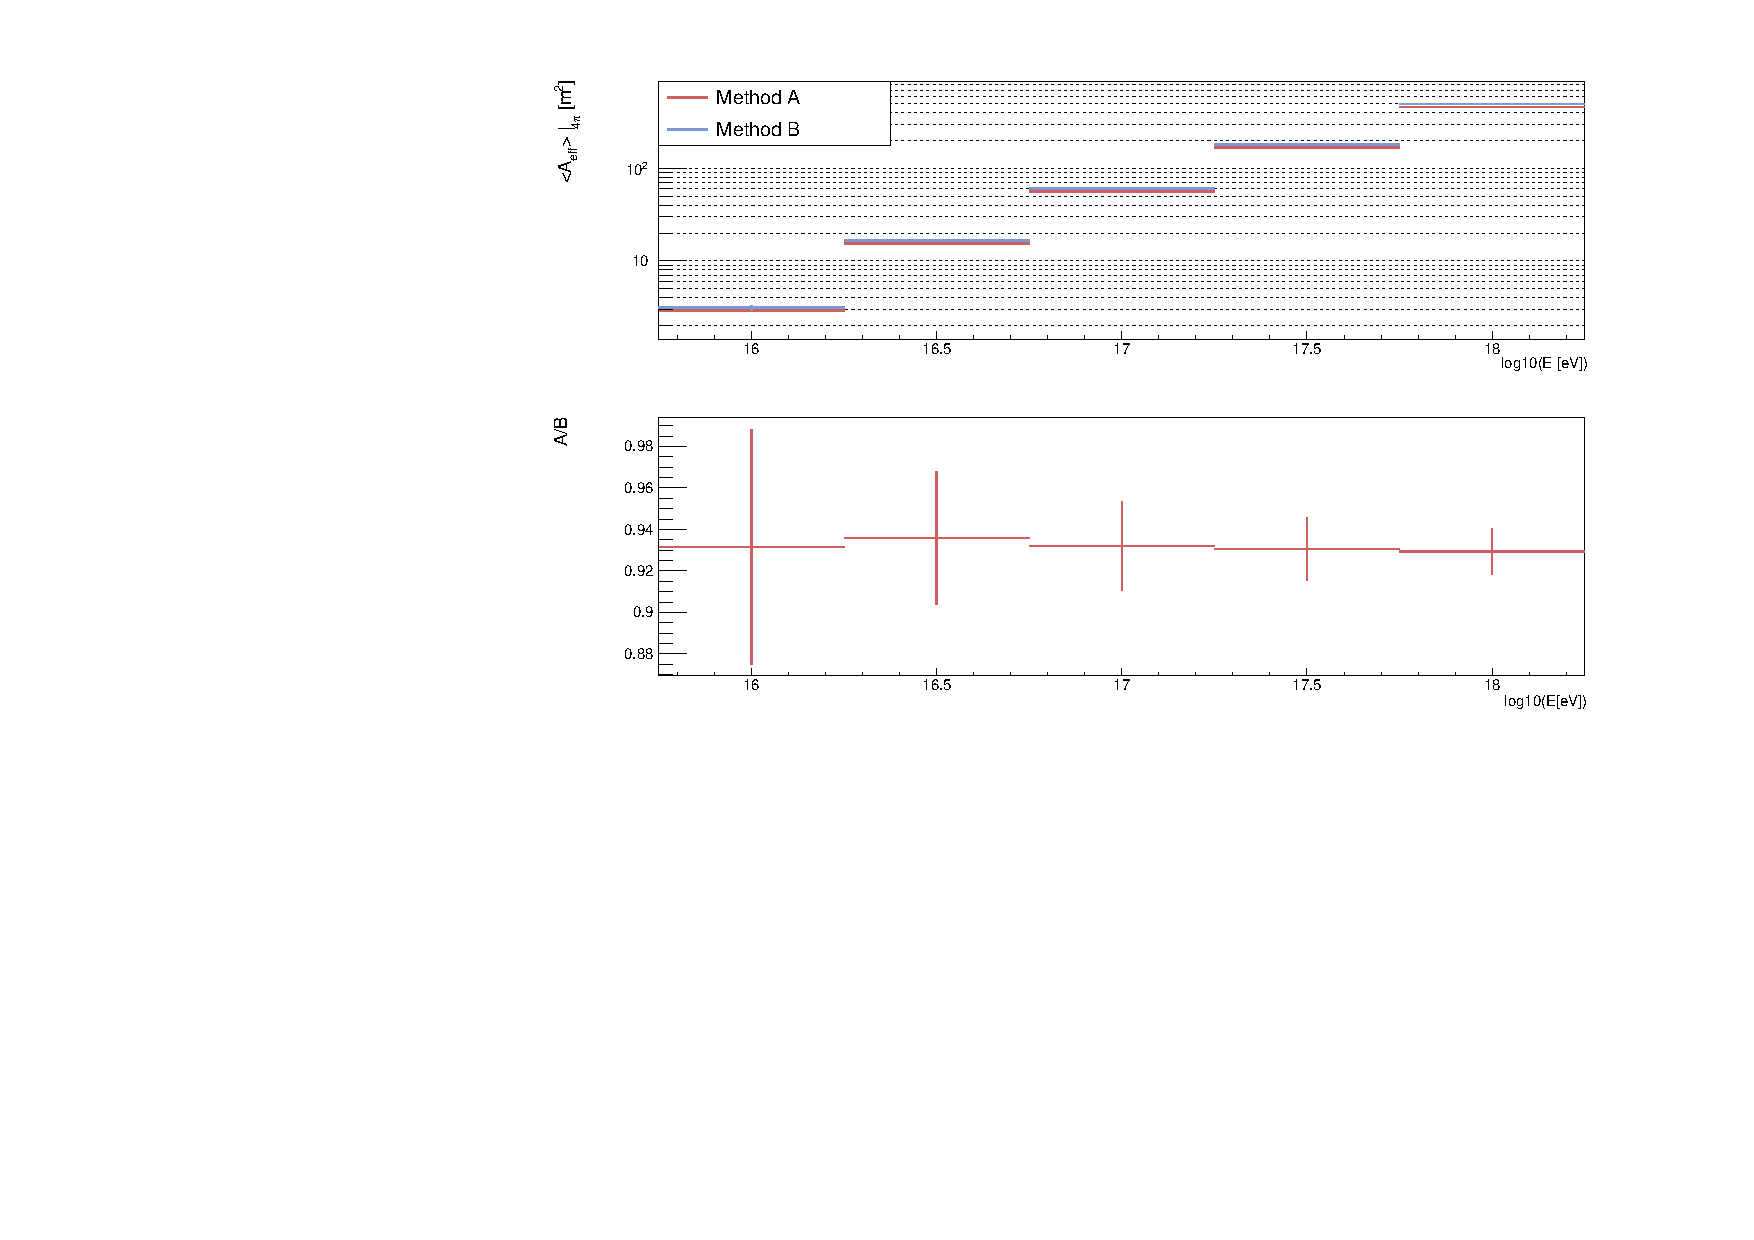
\includegraphics[width=4.5in]{result}

\end{frame} 

\begin{frame}
  \frametitle{Elevation Dependence} 
  \centering
  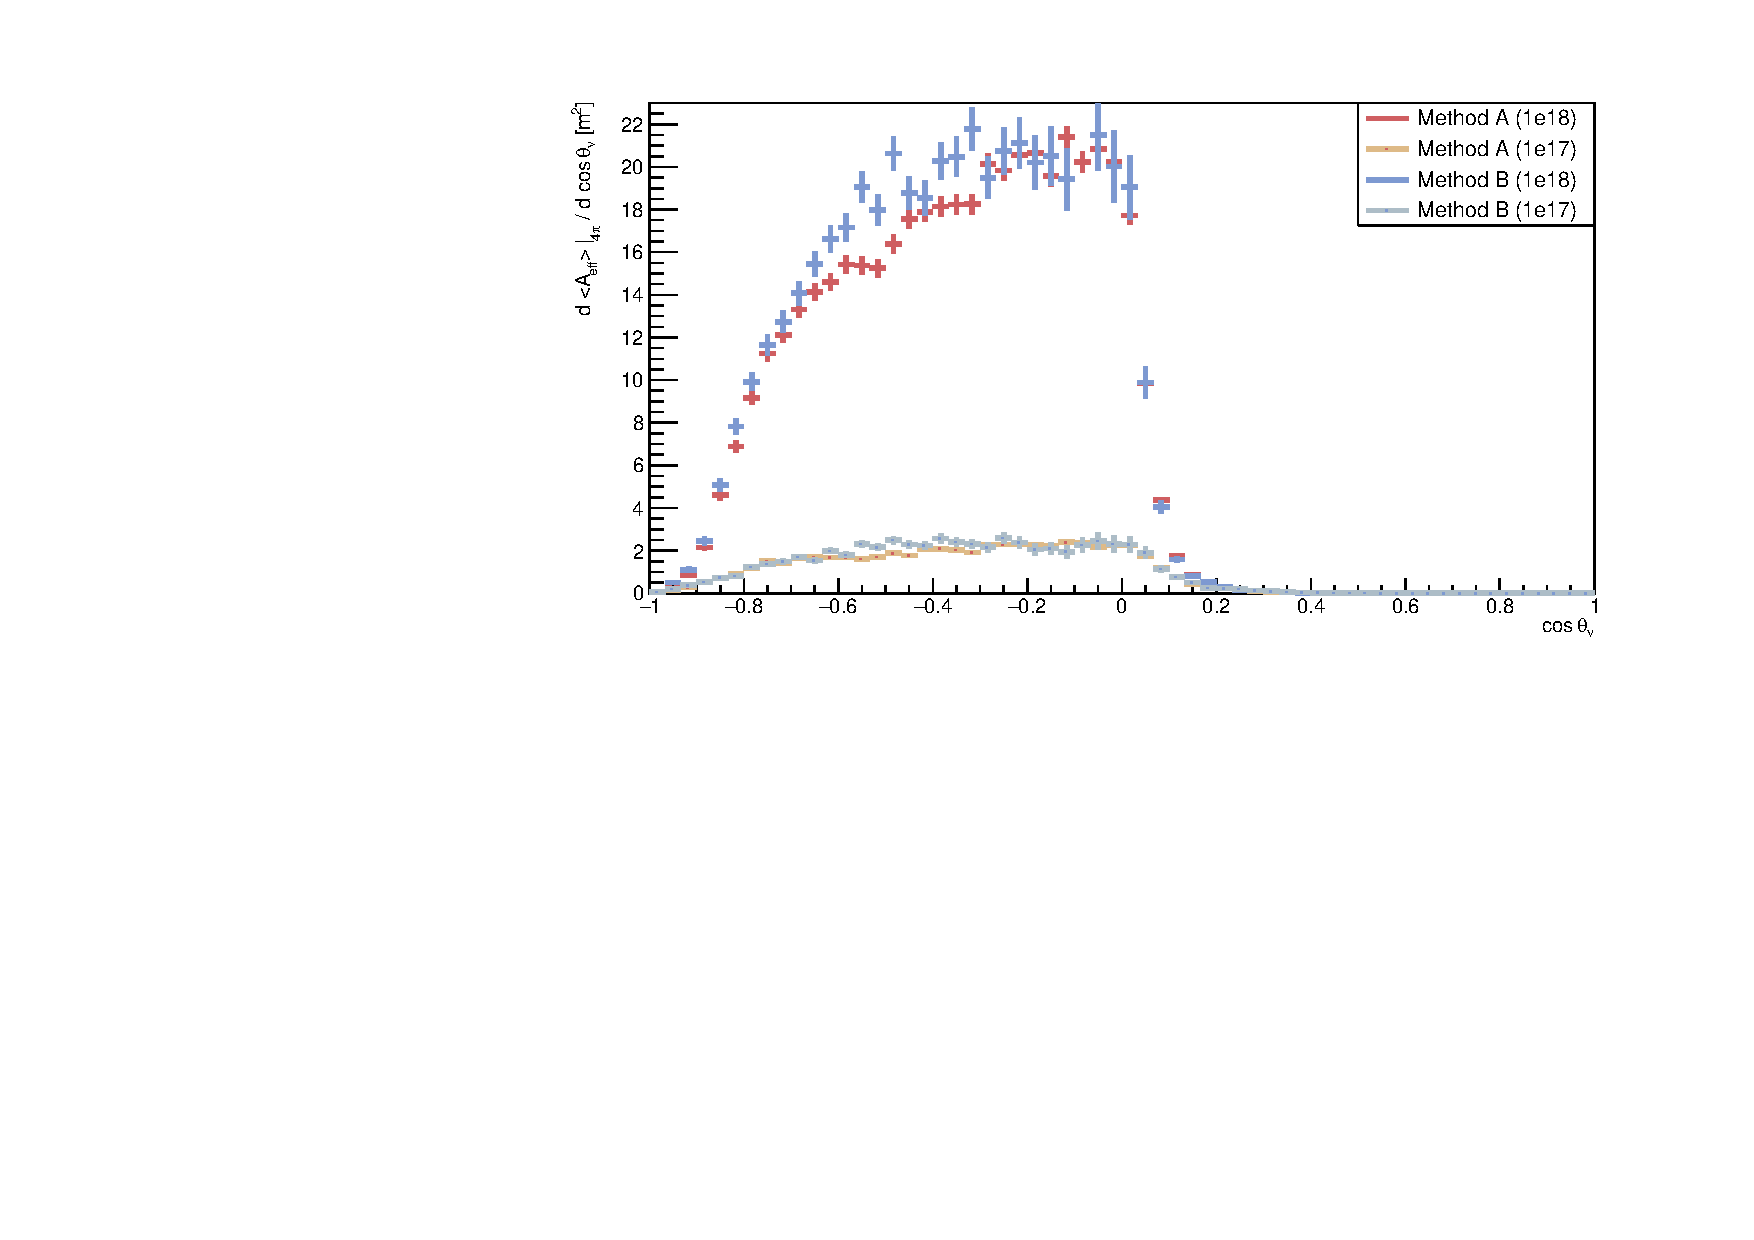
\includegraphics[width=5in]{theta18}
\end{frame} 


\begin{frame}
  \frametitle{Discussion}
  \begin{itemize}
    \item Small, but statistically significant difference between the two generators. 
      \begin{itemize} 
       \item Size of effect on real simulation might be different when including raytracing, more sophisticated trigger.
       \item Size of effect on ANITA, which samples a much narrower angular range with a more complex geometry, might be much larger. 
     \end{itemize} 
    \item Note that since $w_{x} \approx  L_{proj} /L_{int}$, the two expressions for $<A_{eff}>|_{\Omega}$ are not so different. 
    \begin{itemize} 
      \item If instead of a box independent of the incoming angle, we used the projected area for each angle (so no trajectories miss), then you would get almost the same expression as A (since $V_{mc} = <L_{proj}> A_{proj}$), but I don't think you can factor out the integral over $L_{proj}$ out of the other factors in the general case, possibly accounting for the difference.
      \item Suggests possible correction factor of $L_{proj}/ (<L_{proj}>(\theta))$ (or something like that) that might bring the two together (haven't tried this yet). 
    \end{itemize}
\end{itemize} 
\end{frame}


\end{document} 
